\documentclass[a4paper,12pt]{article}
\usepackage[a4paper]{geometry}
\usepackage{color, hyperref}
\usepackage[hypcap]{caption}
\usepackage[utf8]{inputenc}
\usepackage{float}
\usepackage{array}
\usepackage{ulem}
\usepackage{contour}
\usepackage{listings}
\usepackage{booktabs}
\usepackage{multirow}
\usepackage{wrapfig, graphicx}
\usepackage{tikz}

\graphicspath{{./img}}
\hypersetup{
	colorlinks=true,
	breaklinks=true,
	linkcolor=black,
	pdftitle={PolyMessages - Sprint 3}
}

\definecolor{codegreen}{rgb}{0,0.6,0}
\definecolor{codegray}{rgb}{0.5,0.5,0.5}
\definecolor{codepurple}{rgb}{0.58,0,0.82}
\definecolor{backcolour}{rgb}{0.9,0.9,0.9}
\lstdefinestyle{myStyle}{
	backgroundcolor=\color{backcolour},
	commentstyle=\color{codegreen},
	keywordstyle=\color{magenta},
	numberstyle=\tiny\color{codegray},
	stringstyle=\color{codepurple},
	basicstyle=\ttfamily\footnotesize,
	breakatwhitespace=false,
	breaklines=true,
	captionpos=b,
	keepspaces=true,
	showspaces=false,
	showstringspaces=false,
	showtabs=false,
	tabsize=2,
	linewidth=0.95\linewidth,
	xleftmargin=0.2\linewidth,
	% padding=5px
}

\lstset{style=myStyle}


\renewcommand{\ULdepth}{1.8pt}
\contourlength{0.8pt}

\newcommand{\ul}[1]{%
	\uline{\phantom{#1}}%
	\llap{\contour{white}{#1}}%
}

\captionsetup{labelfont={it, bf}, textfont={it}}

\title{PolyMessages | Sprint 3}
\author{Eri Agnese, Marvin Bontemps, Lucas Nouguier}
\date{15 Mai 2022}

\begin{document}
\maketitle
\tableofcontents
\clearpage
\hypersetup{linkcolor=red}

\newgeometry{left=2cm,right=2cm,bottom=2cm, top=1.5cm}

\section{Protocole de communication}
\begin{figure}[h]
	\centering
	\hrulefill\\
	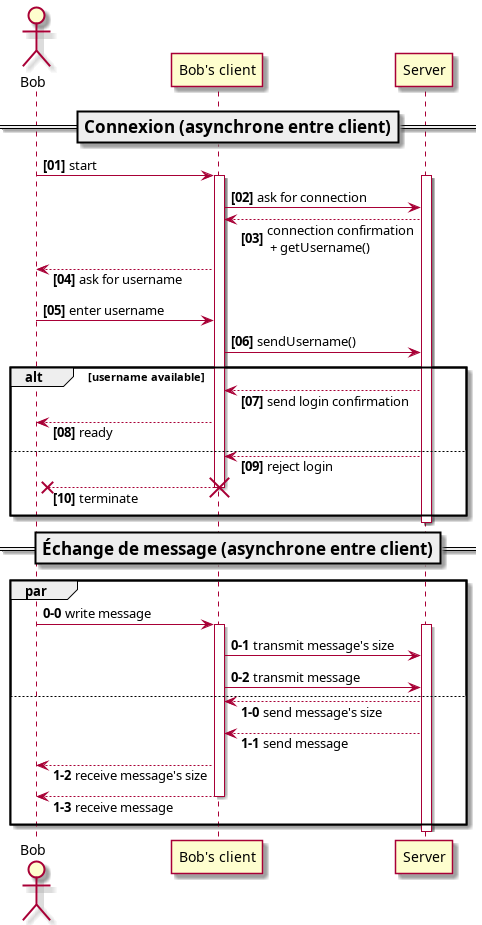
\includegraphics[width=0.45\linewidth]{sequence.png}
	\hfill
	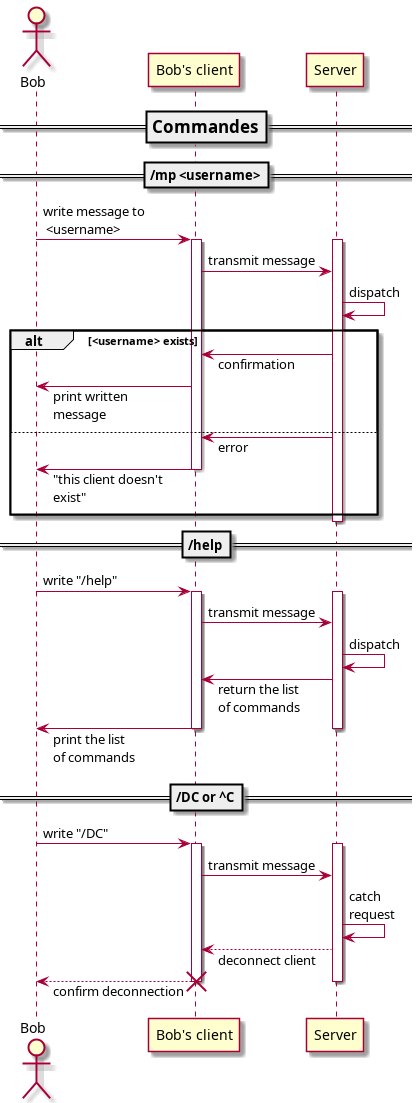
\includegraphics[width=0.4\linewidth]{commands.png}
	\caption{Protocole de communication clients/serveur}
	\hrulefill
\end{figure}

\pagebreak

\begin{figure}[h!]
	\centering
	\hrulefill\\
	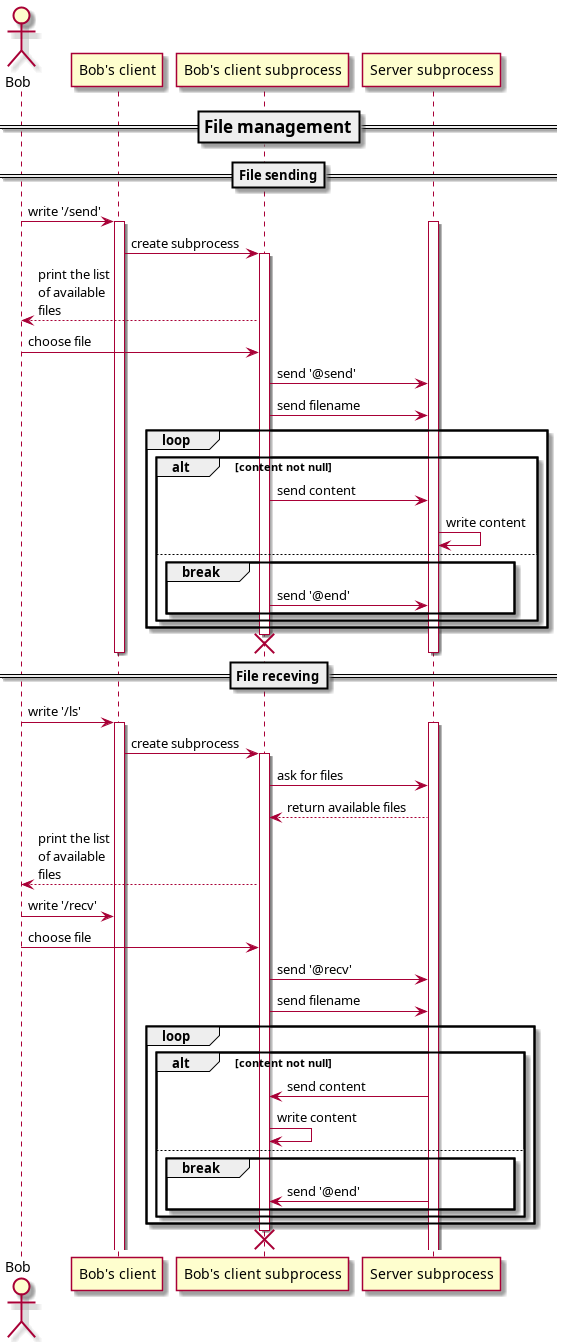
\includegraphics[width=0.6\linewidth]{fileManagement.png}
	\caption{Protocole d'échange de fichiers}
	\hrulefill
\end{figure}

\pagebreak
\section{Architecture}
\begin{figure}[h]
	\centering
	\hrulefill\\
	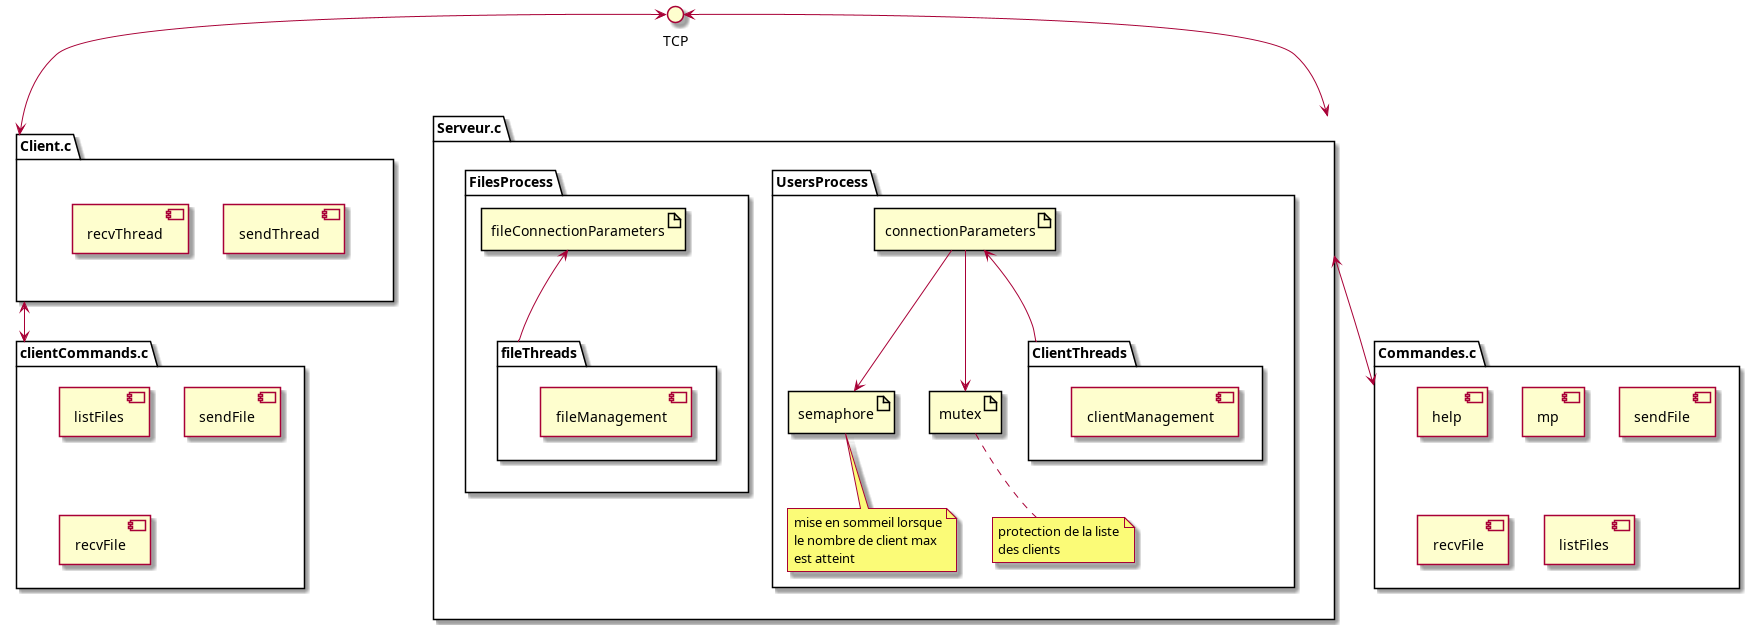
\includegraphics[width=\linewidth]{architecture.png}
	\caption{Architecture de la messagerie}
	\hrulefill
\end{figure}
\section{Répartition du travail}
\begin{wraptable}{r}{0.55\linewidth}
	\vspace{-0.5cm}
	\begin{tabular}{cccc}
		\toprule
		\multirow{2}{*}{Tâches} & \multicolumn{3}{c}{Étudiants}\\
		\cmidrule{2-4}
		& Lucas & Éri & Marvin\\
		\midrule
		Listage fichiers & X\\
		\midrule
		Envoie client$\rightarrow$serveur & X & X & \\
		\midrule
		Reception client$\rightarrow$serveur & & &X\\
		\midrule
		Envoie serveur$\rightarrow$client & & X & X\\
		\midrule
		Reception serveur$\rightarrow$client & & X & X\\
		\midrule
		Intégration & X\\
		\bottomrule
	\end{tabular}
	\caption{Tâche effecutée par étudiant}
	\label{table:repartition}
	\vspace{-0.5cm}
\end{wraptable}
La 3\textsuperscript{ème} version de la messagerie consistait à donner la possibilité d'envoyer des fichiers depuis un répertoire précis. Pour cela, on a permis à l'utilisateur de lister les fichiers disponibles sur le serveur et sur sa machine. Puis on a implementé des fonctions d'envois et de réception.

Pour éviter que les envois soit bloquants (pour le client et pour le serveur), on a choisi de gérer les fichiers :
\begin{itemize}
	\item Sur le client via un processus lourd qui sera lancé à chaque envoi/reception et arrêté lorsque sa tâche sera accomplie
 \item Sur le serveur via un processus lourd (qui lance un serveur écoutant sur un 2nd port) et pour chaque client qui fera une requête sur des fichiers, un thread lui sera associé.
\end{itemize}
Pour l'instant, il n'y a pas de gestion des fichiers de même noms.

\begin{figure}[h]
	\centering
	\hrulefill\\
	\vspace{0.4cm}
	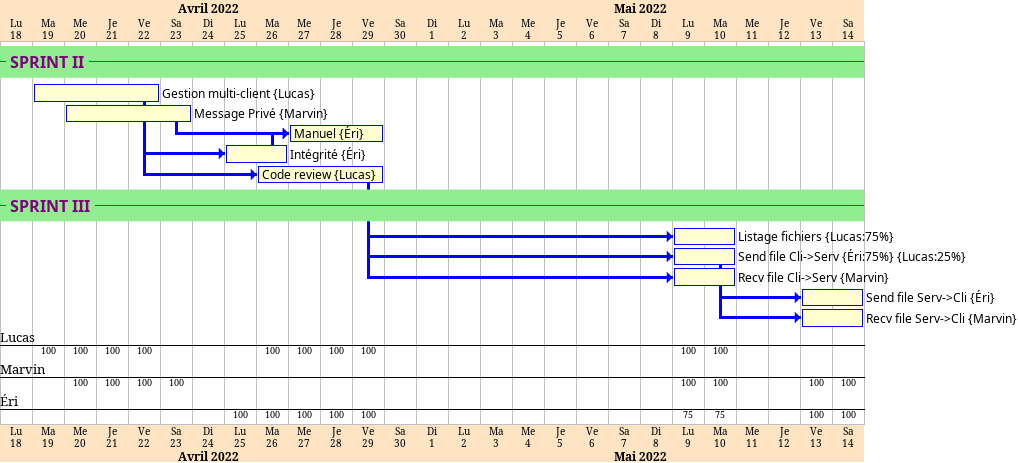
\includegraphics[width=\linewidth]{gantt.png}\\
	\caption{Diagramme de Gantt sur la réalisation du projet}
	\label{fig:gantt}
	\hrulefill
\end{figure}
\pagebreak
\section{Exécution du code}
Pour lancer la messagerie, il faut commencer par compiler et lancer le serveur en spécifiant les 2 ports (1: port d'écoute pour les messages, 2: port d'écoute pour les fichiers)
\begin{figure}[h]
	\centering
	\vspace{-0.1cm}
	\begin{lstlisting}[language=bash, gobble=4]
		[lucas@xps-lucas ~]$ gcc -o server serveur.c commandes.c
		[lucas@xps-lucas ~]$ ./server <PORT1> <PORT2>
	\end{lstlisting}
\end{figure}

\noindent On peut alors lancer les clients en spécifiant les mêmes ports que pour le serveur
\begin{figure}[h]
	\centering
	\vspace{-0.2cm}
	\begin{lstlisting}[language=bash, gobble=4]
		[lucas@xps-lucas ~]$ gcc -o client client.c clientCommands.c
		[lucas@xps-lucas ~]$ ./client <IP> <PORT1> <PORT2>
	\end{lstlisting}
\end{figure}
\section{Difficultés}
\begin{itemize}
	\item On ne peut envoyer qu'un seul fichier par client, après, cela ne fonctionne plus
\end{itemize}
\end{document}